\documentclass[10pt,a4paper]{article}
%standard symbols
\usepackage{amssymb, amsmath, esint, mathrsfs, tipa}
%charts and tables
\usepackage{array, enumitem}
%graphics
\usepackage{graphicx}
%packages for float
\usepackage{wrapfig, placeins, float}
%specialized tools
\usepackage[americanvoltages,RPvoltages]{circuitikz}
%geometry
\usepackage[left=2.0cm, right=2.0cm, top=2.5cm]{geometry}
%code
\usepackage{listings}
%links
\usepackage{hyperref}

\setlength{\textfloatsep}{5pt plus 2pt minus 2pt}
\setlength{\floatsep}{5pt plus 2pt minus 2pt}

\usepackage{color}
\definecolor{dkgreen}{rgb}{0,0.6,0}
\definecolor{gray}{rgb}{.9,.9,.9}
\definecolor{mauve}{rgb}{0.58,0,0.82}
\definecolor{number_blue}{rgb}{0,.557,1}
\definecolor{code_blue}{rgb}{.643,.988,1}
\lstset{
  backgroundcolor=\color{gray},
  keepspaces=true,
  aboveskip=3mm,
  belowskip=3mm,
  showstringspaces=false,
  columns=flexible,
  basicstyle={\small\ttfamily},
  numbers=none,
  numberstyle=\footnotesize\color{number_blue},
  breaklines=true,
  breakatwhitespace=true,
  tabsize=3
}

\begin{document}

\title{ODMB VME Baseline Firmware Guide}
\author{UCSB ODMB Team}
\date{\today}
\maketitle

\section{Test Instructions}

This is document is a guide to using the ODMB7 baseline firmware for testing VME communication and copper (x)DCFEB communication on the ODMB7 version 1 prototype boards. This firmware will confirm if VME signals are properly received and sent to the VME back plane as well as if JTAG signals are properly received and sent to the PPIB/(x)DCFEBs.

Physically, the ODMB should be inserted into an ODMB-compatible slot in a VME crate. There should be a computer with appropriate optical drivers and capable of running some version of Emulib that is connected to and able to control the crate's VCC. This computer should be loaded with the vme\_cli software available at \href{https://github.com/jaebak/vme_cli}{this repository}. There should also be a computer equipped with the Vivado software and connected to the JTAG port of the ODMB via a Xilinx red box. This can be the same or separate from the computer handling VCC communication. Finally, the ODMB should be connected to the two skew-clear cables running to the PPIB. When testing communication with each (x)DCFEB, a powered (x)DCFEB will need to be plugged into the PPIB slot being tested. A diagram of this setup is shown in figure~\ref{fig:vmesetup}.

\begin{figure}[H]
\centering
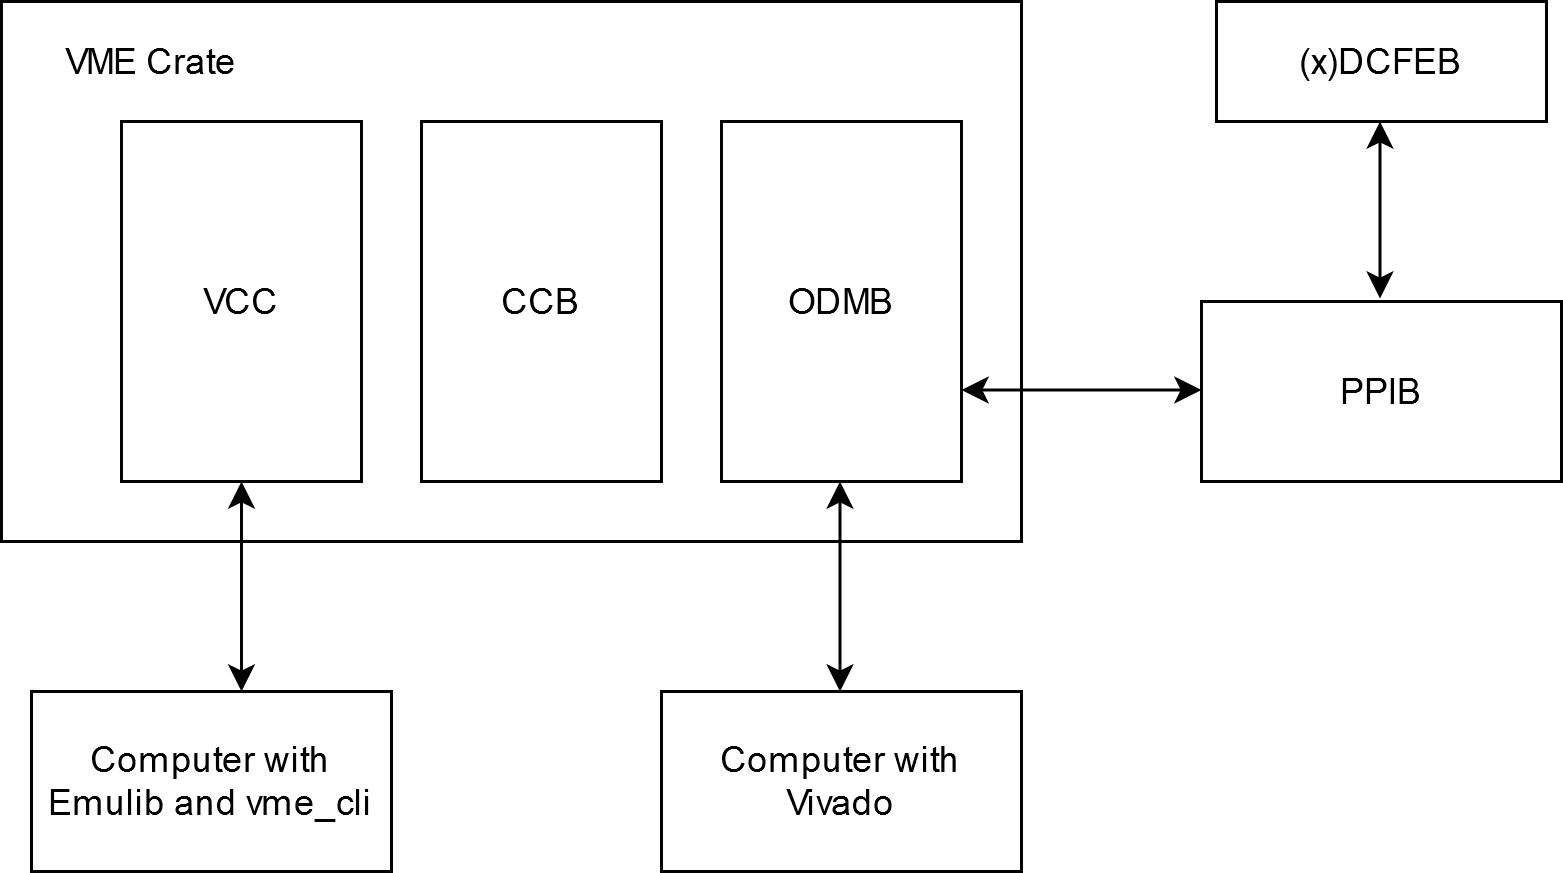
\includegraphics[width= 0.5 \textwidth]{figures/vmesetup.png}
\caption{Test stand configuration for testing the ODMB7 VME baseline firmware.}
\label{fig:vmesetup}
\end{figure}

\begin{figure}[H]
\centering
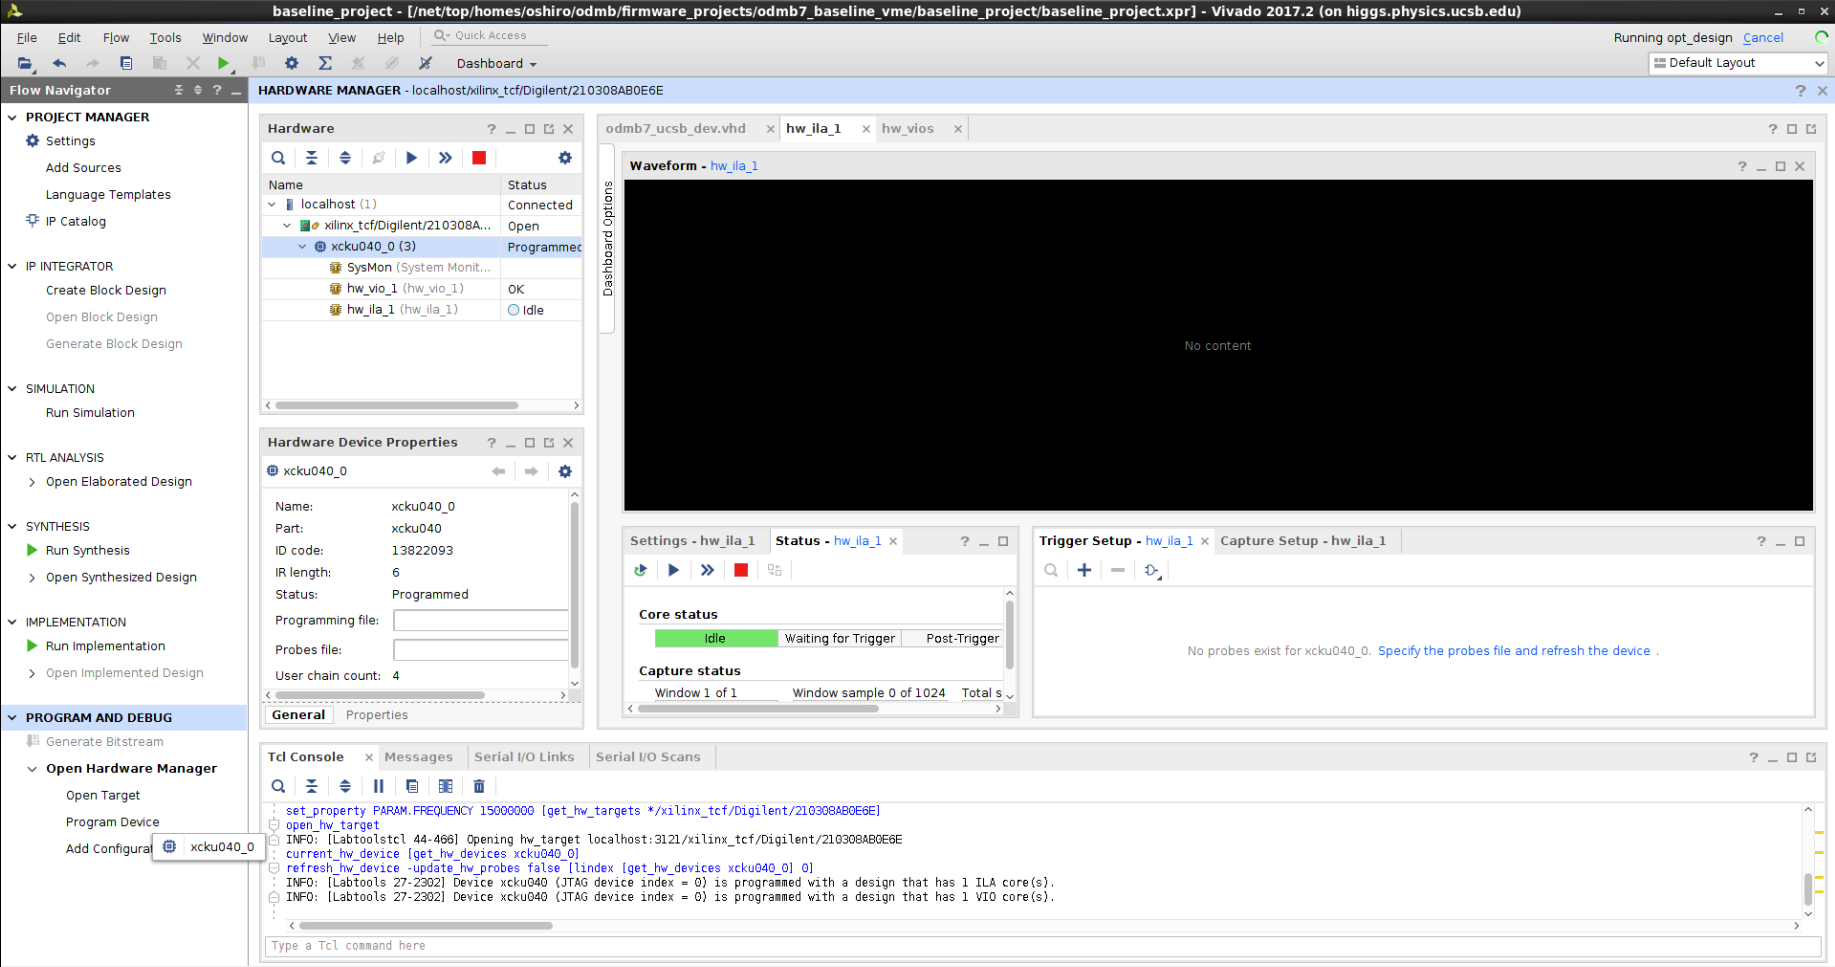
\includegraphics[width= 0.75 \textwidth]{figures/program_step1.png}
\caption{Programming device with Vivado, pictured for KCU105 evaluation board.}
\label{fig:programmingstep1}
\end{figure}

\begin{figure}[H]
\centering
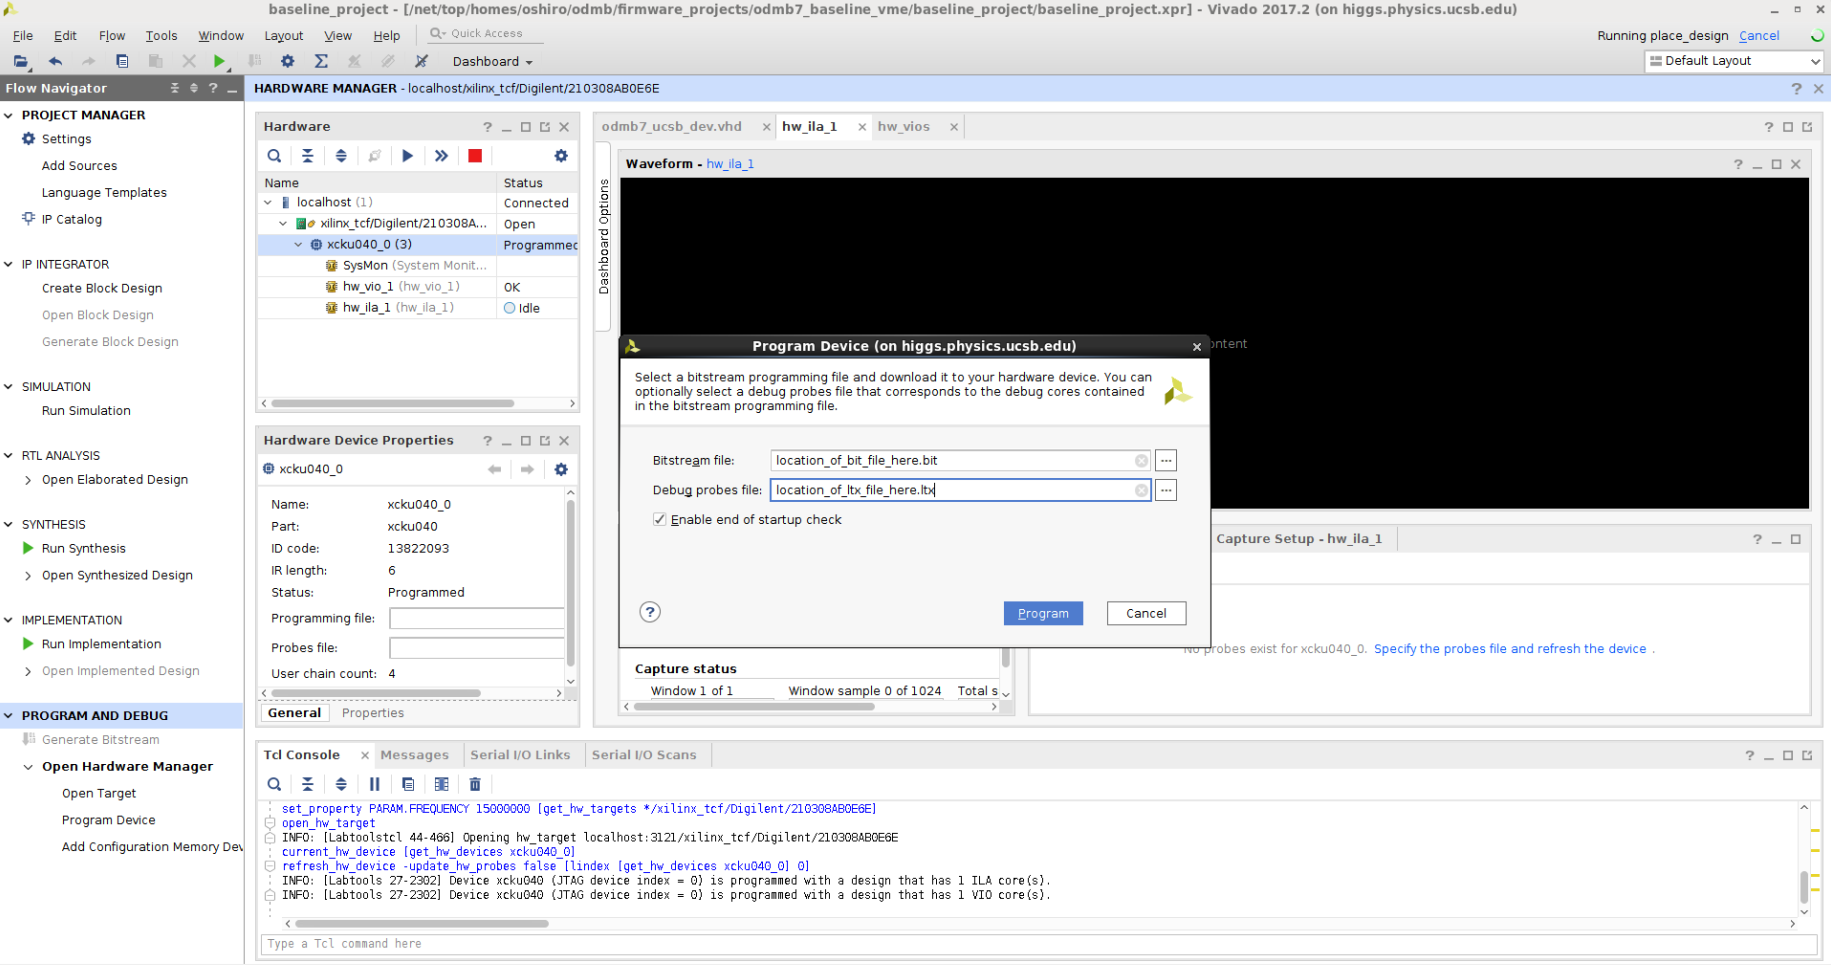
\includegraphics[width= 0.75 \textwidth]{figures/program_step2.png}
\caption{After clicking program device, the bit and ltx files can be specified.}
\label{fig:programmingstep2}
\end{figure}

To begin testing the VME firmware, the prototype boards should be loaded with the provided firmware and the Vivado program equipped with the appropriate test probes. The provided .bit and .ltx files can be loaded as shown in figures~\ref{fig:programmingstep1} and~\ref{fig:programmingstep2}. 

Once the firmware is loaded, VME commands can be sent using the vme\_cli software. After compiling the software with make, a VME command can be issued to the ODMB in a format demonstrated by the following example.

\begin{lstlisting}[label={lst:vmecli}]
./vme_cli --vcc_mac_address 02:00:00:00:00:4A --schar_port 2 --eth_name p5p2 --vme_write_read w --vme_command 1020 --vme_data ff --vme_slot 19
\end{lstlisting}

The VCC MAC address, \texttt{schar\_port}, \texttt{eth\_name}, and VME slot should be adjusted based on the configuration of the host computer and VME crate. The arguments \texttt{vme\_write\_read}, \texttt{vme\_command}, and \texttt{vme\_data} indicate the actual content of the command issued to the ODMB. The \texttt{vme\_write\_read} argument takes on the value \texttt{w} or \texttt{r} to indicate a write or read command respectively. In the case of read commands, no \texttt{vme\_data} needs to be provided. The \texttt{vme\_command} and \texttt{vme\_data} take 16 bit values specified as 4 hex characters. \texttt{vme\_data} values with fewer than 4 characters are interpreted by padding to the left with 0's. Below, commands will be listed in the format \texttt{<vme\_write\_read> <vme\_command> (<vme\_data>) (//comment on command)}.

As a first test, the command \texttt{R 4100} should be issued. The ODMB should respond with the return value \texttt{OD3B}, which will be displayed by the vme\_cli program.

If this is successful, a more complicated series of commands can be issued to read the User code from the (x)DCFEBs. This is given in listing~\ref{lst:usercodedcfeb} for DCFEBs and listing~\ref{lst:usercodexdcfeb} for xDCFEBs. The two \texttt{R 1014} commands will return the usercode, which should be \texttt{DCFEB\#\#\#} where the \#'s depend on the firmware version of the (x)DCFEB. Note that the lower 16 bits get returned first.

\begin{lstlisting}[label={lst:usercodedcfeb}]
W 1018 0000 //reset DCFEBs
W 1020 #    //Select DCFEBs, use #=01, 02, 04, 08, 10, 20, or 40 to select DCFEB 1, 2, 3, 4, 5, 6, or 7 respectively
W 191C 3C8  //shift instruction "read usercode"
W 1F04 0000 //shift 16 upper data bits
R 1014      //read retrieved data bits
W 1F08 0000 //shift 16 lower data bits
R 1014      //read retrieved data bits
\end{lstlisting}

\begin{lstlisting}[label={lst:usercodexdcfeb}]
W 1018 0000 //reset DCFEBs
W 1020 #    //Select DCFEBs, use #=01, 02, 04, 08, 10, 20, or 40 to select DCFEB 1, 2, 3, 4, 5, 6, or 7 respectively
W 1934 3C8  //shift instruction "read usercode"
W 1F30 FFFF //bypass instruction to other xDCFEB devices
W 1F30 FFFF //bypass instruction to other xDCFEB devices
W 1F30 FFFF //bypass instruction to other xDCFEB devices
W 1338 F    //bypass instruction to other xDCFEB devices
W 1F04 0000 //shift 16 upper data bits
R 1014      //read retrieved data bits
W 1F08 0000 //shift 16 lower data bits
R 1014      //read retrieved data bits
\end{lstlisting}

If the returned values from \texttt{R 4100} or \texttt{R 1014} are not as expected, more information on debugging is given in the next section.

\section{Debugging}

\subsection{Check Clocks}

The first check to perform if the \texttt{R 4100} command fails is to check the ODMB clocks. If the CMS clock is not received from the CCB or if the clock manager is not functional, the ODMB firmware will not be able to handle VME communication. To diagnose these problems, one can first run the ILA un-triggered. If the ILA does not respond, this is indicative of no clock signal, which can be caused by either not receiving the CMS clock from the CCB or a malfunction of the clock manager in firmware.

If it is suspected that the CMS clock is not being received, an alternative firmware version with the ILA directly reading the CMS clock signal can be generated. Alternatively, the firmware can be replaced with an alternate version that uses the clock from the on-board clock synthesizer, which must be configured using appropriate software. Failure to see the CMS clock directly and success with the alternate firmware indicates a problem in receiving the clock from the CCB.

If the alternative firmware that reads the clock signal directly from the CCB demonstrates the clock is being received, then the clock manager module in the firmware is likely at fault and firmware debugging is required.

\subsection{Check VME Signals}

If the clock signals look as expected, the next debugging step is to check that VME signals are being sent/received. To diagnose VME problems, the VME crate should be restarted and the ODMB ILA equipped with the VME signals listed in table~\ref{tab:vmesignals}. This table also lists the expected behavior of the signals and their response to a \texttt{R 4100} command in simulation is shown in figure~\ref{fig:vmecommand}. Once the ILA is equipped with the appropriate signals, it should be triggered on \texttt{vme\_as\_b}=0. Once the ILA is armed, a \texttt{R 4100} command should be issued from vme\_cli.

The first thing to check are the strobes and dtack. The VCC should pull \texttt{vme\_as\_b} low, then both bits of \texttt{vme\_ds\_b}. Shortly after \texttt{vme\_ds\_b} is pulled low, the \texttt{strobe} signal become 1. After some time, the ODMB should pull \texttt{vme\_dtack\_v6\_b} low, and the VCC should de-assert \texttt{vme\_ds\_b}, then \texttt{vme\_as\_b}. If \texttt{vme\_as\_b} or \texttt{vme\_ds\_b} is never pulled low, and \texttt{vme\_dir} is low, there may be some problem receiving the appropriate signal, which could be caused by ICs or traces on the ODMB. Further debugging may be performed with an oscilloscope on appropriate IC legs. If \texttt{vme\_as\_b} and \texttt{vme\_ds\_b} are pulled low but \texttt{strobe} never goes high, the other \texttt{vme\_} signals listed in table~\ref{tab:vmesignals} should be checked against their expected values. If these match their expected values, additional firmware will need to be generated to debug firmware issues.

If the correct sequence of strobes and dtack is observed, then the VME command is being received by the ODMB and the signals \texttt{vme\_data\_out}, \texttt{vme\_tovme}, and \texttt{vme\_doe\_b} should be checked against their expected values. If these signals match their expected values, external ICs and signal traces may need to be debugged. 

If \texttt{vme\_data\_out} is incorrect or if \texttt{strobe} is asserted but \texttt{vme\_dtack\_v6\_b} never goes low, it is likely that the VME modules in the firmware are at fault. The \texttt{dummy\_confregs} module that handles the \texttt{R 4100} command is very simple and thus not expected to fail. Information on debugging the \texttt{cfebjtag} module is given in the next section.

\begin{table}[H]
\centering
\resizebox{\textwidth}{!}{%
\begin{tabular}{ l|l l} 
Signal& Long name& Expected behavior\\ \hline
\texttt{vme\_data\_in\_buf}& Data in& Value passed by vme\_cli for write commands.\\ 
\texttt{vme\_data\_out\_buf}& Data out& Value returned by ODMB.\\ 
\texttt{vme\_crate\_addr}& Address& The slot number should match the bitwise inverse of \texttt{vme\_ga\_b} when \texttt{vme\_as\_b} goes low.\\ 
\texttt{vme\_cmd}& Command& Should match value passed by vme\_cli.\\ 
\texttt{vme\_am}& Address Modifier. & When \texttt{vme\_as\_b} goes low, this should be 111X10 or 111X01. \\ 
\texttt{vme\_gap\_b}& Geographical address parity. &Should be 1 if an odd number of bits in ga are 0 and 0 otherwise.\\ 
\texttt{vme\_ga\_b}& Geographical address.& Should correspond to the VME slot used.\\ 
\texttt{vme\_as\_b}& Address strobe.& Should go low to indicate address ready to read.\\ 
\texttt{vme\_ds\_b}& Data strobe.& Both bits should go low after \texttt{vme\_as\_b} to indicate data ready to read.\\ 
\texttt{vme\_sysfail\_b}& Sysfail.& Should be 1.\\ 
\texttt{vme\_berr\_b}& Bus Error.& Should be 1, but doesn't matter for ODMB.\\ 
\texttt{vme\_iack\_b}& Interrupt acknowledge.& Should be 1.\\ 
\texttt{vme\_lword\_b}& Load word.& Should be 1 when \texttt{vme\_as\_b} goes low.\\ 
\texttt{vme\_write\_b}& Write.& Should be 0 for write commands and 1 for read commands.\\ 
\texttt{vme\_dtack\_v6\_b}& Data acknowledge.& Should be issued by ODMB some time after receiving \texttt{vme\_ds\_b} low.\\ 
\texttt{vme\_dir}& To VME& Should be go high when read commands are sent and low otherwise.\\
\texttt{vme\_doe\_b}& Output Enable& Should go low when read commands are sent.\\
\texttt{strobe}& Stobe& Should go high shortly after \texttt{vme\_ds\_b} goes low.\\
\end{tabular}%
}
\caption{Signals in VME interface}
\label{tab:vmesignals}
\end{table}

\begin{figure}[H]
\centering
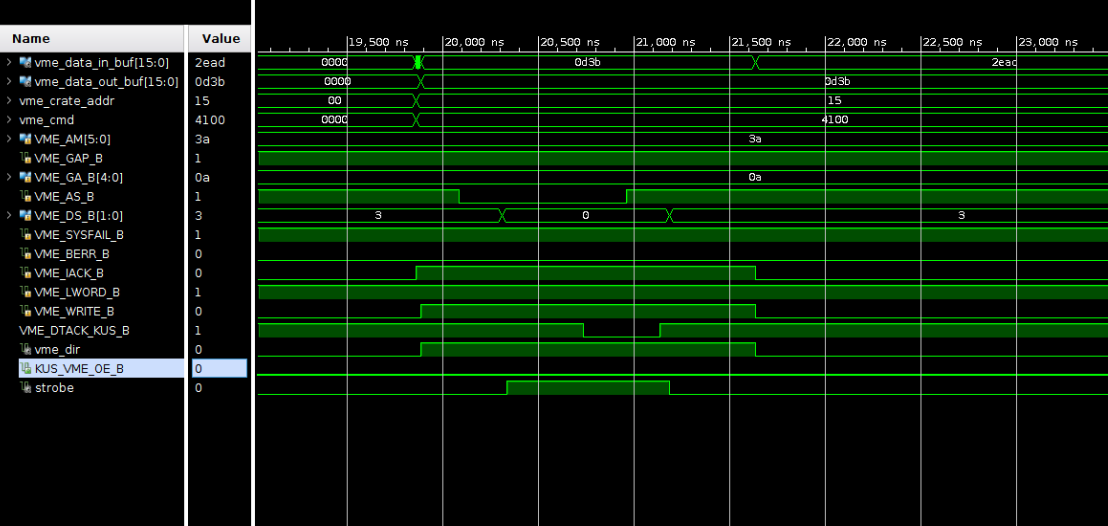
\includegraphics[width= 1.0 \textwidth]{figures/vmeexample.png}
\caption{Simulated ODMB response to VME command \texttt{R 4100}. Note that in simulation \texttt{2EAD} appears on the \texttt{vme\_data\_in} line while in the real ODMB, a value of \texttt{0000} is expected.}
\label{fig:vmecommand}
\end{figure}

\subsection{Check CFEBJTAG}

If the user code can not be successfully read back from the (x)DCFEBs, the first thing to check are the JTAG communication lines. These signals are \texttt{tms}, \texttt{tck}, \texttt{tdi}(selected (x)DCFEB index), and \texttt{tdo}(selected (x)DCFEB index), and are listed along with the other signals relevant to \texttt{cfebjtag} in table~\ref{tab:jtagsignals}. Note that the signals in the ILA are prefixed with \texttt{dcfeb\_}. Their expected behavior along with that of other \texttt{cfebjtag} signals is shown in figures~\ref{fig:jtag1018} through~\ref{fig:jtag1f08}.

As a first qualitative check, after each \texttt{W 1X0Y}, \texttt{W 1X1Y}, or \texttt{W 1X3Y} command, the \texttt{tms} signal and the \texttt{tck} only for the selected (x)DCFEB should respond with some pattern. This can be observed by again triggering on \texttt{vme\_as\_b}=0. If they do not respond, this indicates a bug in generating a \texttt{busy} signal or appropriate \texttt{tms} response and the appropriate paragraph below should be referenced. If other \texttt{tck} clocks are running, this indicates a problem in selecting the correct dcfeb and the \texttt{selfeb} signal should be monitored as discussed below.

If \texttt{tms} and \texttt{tck} seem to respond to appropriate commands, one should check that the correct \texttt{tdo} bits are being returned from the (x)DCFEBs. When the \texttt{W 1F04} and \texttt{W 1F08} commands are issued, one can check the value of \texttt{tdo} on rising edges of \texttt{tck} after \texttt{tms} has been 0 for two cycles up to and including the first \texttt{tck} edge for which \texttt{tms} is 1. The bits should be \texttt{DCFEB\#\#\#} noting that the shifted bits on \texttt{tdo} appear in reverse order.

If the \texttt{tdo} bits are not correct, it may be necessary to inspect each \texttt{W 1X0Y}, \texttt{W 1X1Y}, and \texttt{W 1X3Y} command issued in detail. Figures~\ref{fig:jtag1018} through \ref{fig:jtag1f08} show the expected behavior for each command. To compare to the figures, check the value of \texttt{tdi} and \texttt{tms} against the values shown in the figures for each rising edge of \texttt{tck}. If the \texttt{tdi} or \texttt{tms} are incorrect, this indicates a bug in the logic that generates the \texttt{tms} patterns or transfers the input to \texttt{tdi}.

If the \texttt{tms} clock never begins running after a (x)DCFEB communication command is issued, this indicates either a problem in generating a \texttt{busy} signal or a failure to select any (x)DCFEBs. To diagnose the prior issue, check the \texttt{strobe}, \texttt{load}, \texttt{busy}, and \texttt{tck\_global} signals after issueing a command. The load should go high once after receiving \texttt{strobe} high. If this does not happen, check that \texttt{vme\_cmd} is correct. After load goes high, \texttt{busy} should go high until the communication is finished and while \texttt{busy} is running, \texttt{tck\_global} should be running. If this does not happen, more debugging will be required for the \texttt{busy} logic. 

If multiple \texttt{tms} clocks are running or if \texttt{tck\_global} is running but no other \texttt{tck} signals, this indicates a problem with selecting (x)DCFEBs. One should check the \texttt{selfeb}signal after issuing a \texttt{W 1020} to see if updates to reflect selected (x)DCFEBs. The command \texttt{R 1024} can also be used to read back the currently selected (x)DCFEBs to check. After issuing a \texttt{W 1020} command, one run the ILA untriggered or issue \texttt{R 1024} to see if the selected (x)DCFEBs are still selected. If not, it is likely the ODMB received a spurious reset, and additional firmware should be made to investigate spurious reset signals.

If \texttt{tms} is not generated properly for a particular command, signals involved in \texttt{tms} pattern generation should be investigated. In particular, for \texttt{W 1Y1C} and \texttt{W 1Y34}, the \texttt{shihead} signal should be asserted to shift the instruction header before shifting data. For the \texttt{W 1Y04} command, the \texttt{shdhead} signal should be asserted to shift the data header. For all JTAG shift commands, the \texttt{shdata} signal should be asserted to shift the \texttt{tdi}/\texttt{tdo} data. Then, for \texttt{W 1Y1C}, \texttt{W 1Y38}, and \texttt{W 1Y08} commands, the \texttt{shtail} signal should be asserted to shift the tailer at the end of the shifting. If any of these signals are not asserted, additional firmware should be generated to analyze the VHDL logic generating the signal in question. If the signals are generated, but the \texttt{tms} or \texttt{tdi} patterns are not correct, additional firmware should be generated to analyze the shifting logic.

\begin{table}[H]
\centering
\resizebox{\textwidth}{!}{%
\begin{tabular}{ l|l l} 
Signal& Description& Expected behavior\\ \hline
\texttt{dcfeb\_tms}& JTAG Control& While \texttt{tck} is running, this should various values depending on command issued. See figures~\ref{fig:jtag1018}\\
                        & & through~\ref{fig:jtag1f08} for expected behavior for DCFEB commands\\
\texttt{dcfeb\_tck}& JTAG Clock& After a \texttt{W 1X0Y}, \texttt{W 1X1Y}, or \texttt{W 1X3Y} command, the TCK for the selected\\
                      & & (x)DCFEB should oscillate for several cycles\\ 
\texttt{dcfeb\_tdi}& JTAG Input& When \texttt{tck} is running, the bits matching the provided \texttt{vme\_data} should be seen.\\
\texttt{dcfeb\_tdo}& JTAG Output& During the final \texttt{W 1F04} and \texttt{W 1F08} commands, the \texttt{tdo} signal for the\\
                       & & selected (x)DCFEB should be the bits for its usercode.\\
\texttt{load}& Load& Should go high once for each (x)DCFEB communication command issued.\\
\texttt{busy}& Busy& Should be asserted while JTAG shifts in progress.\\
\texttt{tck\_global}& Global JTAG clock.& Should be sent to selected (x)DCFEB(s) as \texttt{tck}.\\
\texttt{selfeb}& Selected (x)DCFEB& Should match selected (x)DCFEB(s) after issuing \texttt{W 1020} command.\\
\texttt{shihead}& Shift instruction header.& Should go high for \texttt{W 1Y1C} and \texttt{W 1Y34} commands.\\
\texttt{shdhead}& Shift data header.& Should go high for \texttt{W 1Y04} commands.\\
\texttt{shdata}& Shift data.& Should go high for all JTAG shift commands commands.\\
\texttt{shtail}& Shift tailer.& Should go high for \texttt{W 1Y08}, \texttt{W 1Y1C}, and \texttt{W 1Y38} commands.\\
\end{tabular}%
}
\caption{Signals related to JTAG debugging}
\label{tab:jtagsignals}
\end{table}

\begin{figure}[H]
\centering
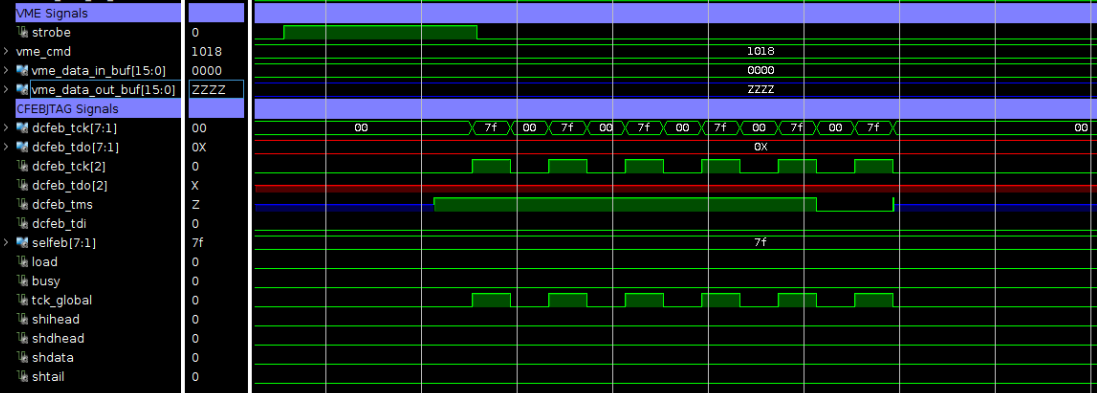
\includegraphics[width= 1.0 \textwidth]{figures/cfebjtag_1018.png}
\caption{Simulated ODMB response to VME command \texttt{W 1018 0000}. Note that this JTAG reset commands causes \texttt{tck} for each (x)DCFEB to run.}
\label{fig:jtag1018}
\end{figure}

\begin{figure}[H]
\centering
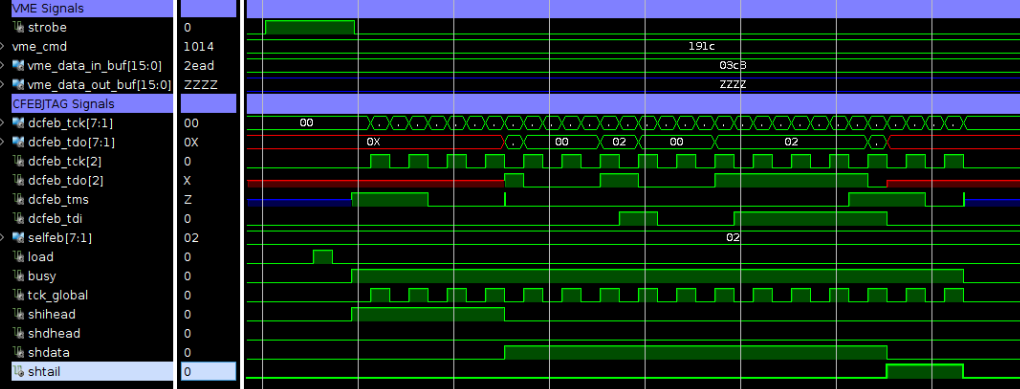
\includegraphics[width= 1.0 \textwidth]{figures/cfebjtag_191c.png}
\caption{Simulated ODMB response to VME command \texttt{W 191C 03C8}. In this example, DCFEB 2 is selected. The \texttt{tdo} signals are unimportant and may differ for real DCFEBs.}
\label{fig:jtag191c}
\end{figure}

\begin{figure}[H]
\centering
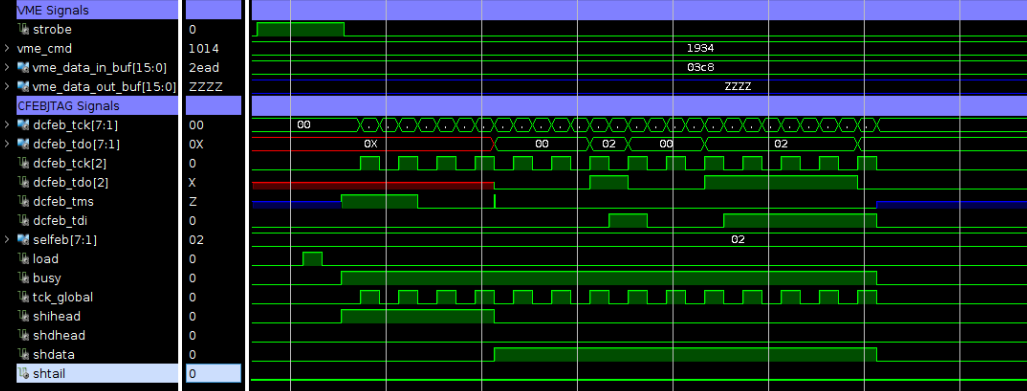
\includegraphics[width= 1.0 \textwidth]{figures/cfebjtag_1934.png}
\caption{Simulated ODMB response to VME command \texttt{W 1934 03C8}. In this example, xDCFEB 2 is selected. The \texttt{tdo} signals are unimportant and may differ for real xDCFEBs.}
\label{fig:jtag1934}
\end{figure}

\begin{figure}[H]
\centering
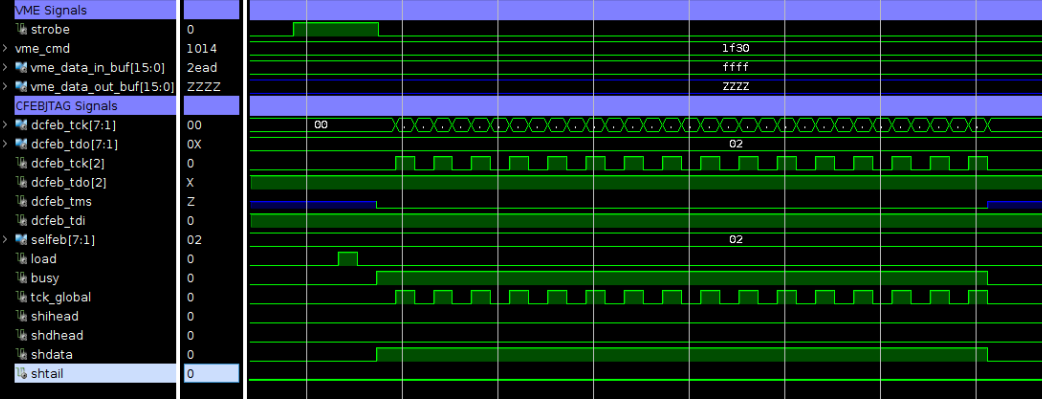
\includegraphics[width= 1.0 \textwidth]{figures/cfebjtag_1f30.png}
\caption{Simulated ODMB response to VME command \texttt{W 1F30 FFFF}. In this example, xDCFEB 2 is selected. The \texttt{tdo} signals are unimportant and may differ for real xDCFEBs.}
\label{fig:jtag1f30}
\end{figure}

\begin{figure}[H]
\centering
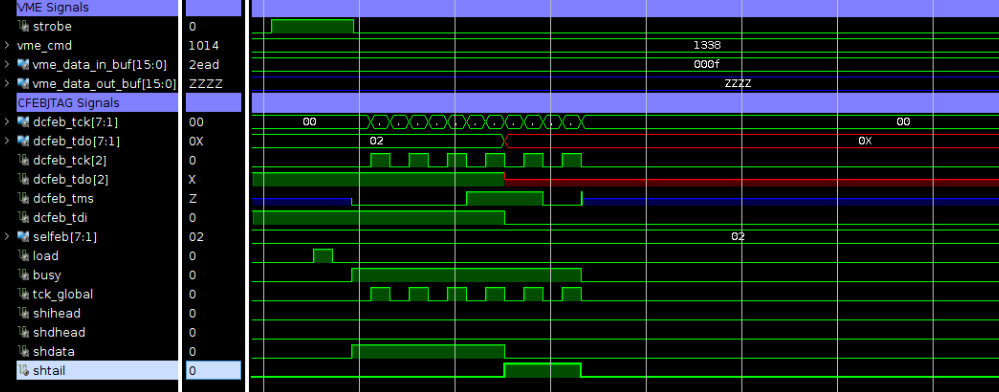
\includegraphics[width= 1.0 \textwidth]{figures/cfebjtag_1338.png}
\caption{Simulated ODMB response to VME command \texttt{W 1338 000F}. In this example, xDCFEB 2 is selected. The \texttt{tdo} signals are unimportant and may differ for real xDCFEBs.}
\label{fig:jtag1338}
\end{figure}

\begin{figure}[H]
\centering
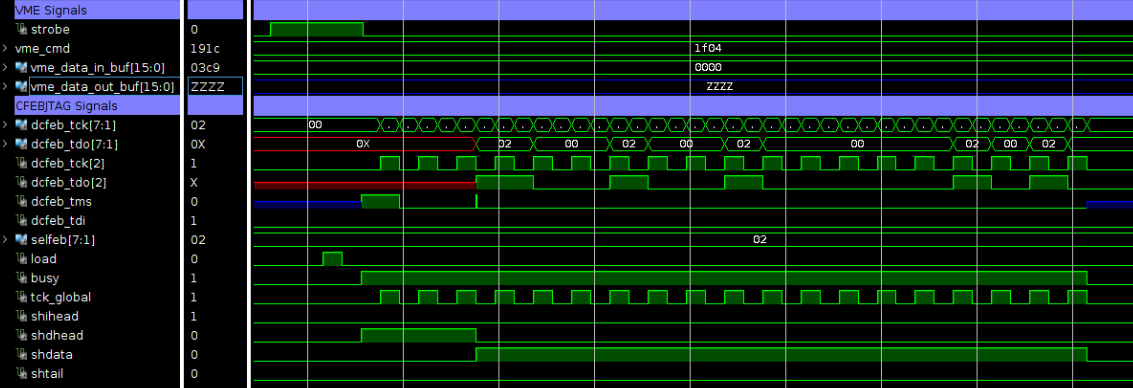
\includegraphics[width= 1.0 \textwidth]{figures/cfebjtag_1f04.png}
\caption{Simulated ODMB response to VME command \texttt{W 1F04 0000}. In this example, xDCFEB 2 is selected. The \texttt{tdo} signal in simulation is \texttt{A093} rather than \texttt{B\#\#\#}
expected for a real (x)DCFEB.}
\label{fig:jtag1f04}
\end{figure}

\begin{figure}[H]
\centering
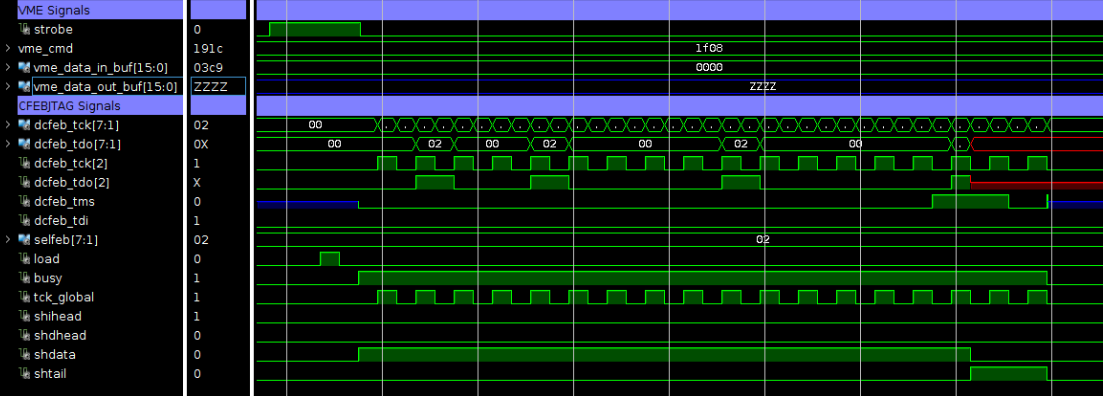
\includegraphics[width= 1.0 \textwidth]{figures/cfebjtag_1f08.png}
\caption{Simulated ODMB response to VME command \texttt{W 1F08 0000}. In this example, xDCFEB 2 is selected. The \texttt{tdo} signal in simulation is \texttt{0424} rather than \texttt{DCFE}
expected for a real (x)DCFEB.}
\label{fig:jtag1f08}
\end{figure}

\end{document}
